\documentclass[conference]{IEEEtran}

\usepackage[spanish]{babel}
\usepackage[utf8]{inputenc}
\usepackage{graphicx}
\usepackage{url}
\usepackage{hyperref}
\usepackage{subfig}
\usepackage{float}
\usepackage{amsmath,amssymb,amsfonts}
\usepackage{booktabs}
\usepackage{array}

\usepackage{datetime}
\newdateformat{specialdate}{\twodigit{\THEDAY}-\twodigit{\THEMONTH}-\THEYEAR}
\date{\specialdate\today}

\usepackage[hyphenbreaks]{breakurl}


\renewcommand\spanishtablename{Tabla}
\renewcommand\spanishfigurename{Figura}

\begin{document}

\title{Reporte de Proyecto Museo VR con Visor Estereoscópico, Navegabilidad y Corrección de Movimiento en Android}

\author{
\IEEEauthorblockN{Ezequiel Torres-Desilos\\
Eduardo Rodrigo Perez-Casas\\
Carlos Alejandro Méndez-Reyes\\
Kenia Elizondo-Maravilla\\
Angel Osmar Perez-Guevara*}
\IEEEauthorblockA{
*Ingeniería en Tecnologías de la Información\\
Universidad Politécnica de Victoria
}
}

\maketitle

\begin{abstract}
En este proyecto se desarrolló y ajustó una aplicación móvil de museo virtual en Android con visualización estereoscópica tipo visor VR. El trabajo se centró en mejorar la experiencia de navegación, corregir el desplazamiento fuera de plano al realizar movimientos verticales con la vista y adaptar un visor oscuro con zona central de observación para cada ojo. La aplicación utiliza renderizado gráfico, seguimiento de orientación y una interfaz dividida en dos vistas para simular la percepción binocular en un entorno inmersivo.
\end{abstract}

\section{Introducción}

La realidad virtual en dispositivos móviles permite representar entornos digitales inmersivos mediante el uso de sensores de orientación, renderizado en tiempo real y división estereoscópica de la pantalla. En Android, este tipo de aplicaciones puede implementarse con OpenGL ES para dibujar escenas 3D y con los sensores del dispositivo para modificar la cámara de acuerdo con el movimiento de la cabeza \cite{androidopengl,androidsensors}.

El presente proyecto corresponde a una aplicación de museo virtual donde el usuario puede observar un espacio arquitectónico simulado mediante un visor VR. A partir del proyecto base, se realizaron ajustes relacionados con la navegabilidad mediante control, la corrección del movimiento fuera de plano al voltear hacia arriba y la integración visual de un visor similar al utilizado en la aplicación de referencia UPV.

El propósito principal fue mejorar la estabilidad visual del recorrido y lograr que la experiencia se presentara de forma clara en ambas vistas del visor. Para ello, se revisó el comportamiento de la cámara, la composición de la escena y la superposición del marco negro que delimita el área visible para cada ojo.

\begin{figure}[H]
\centering
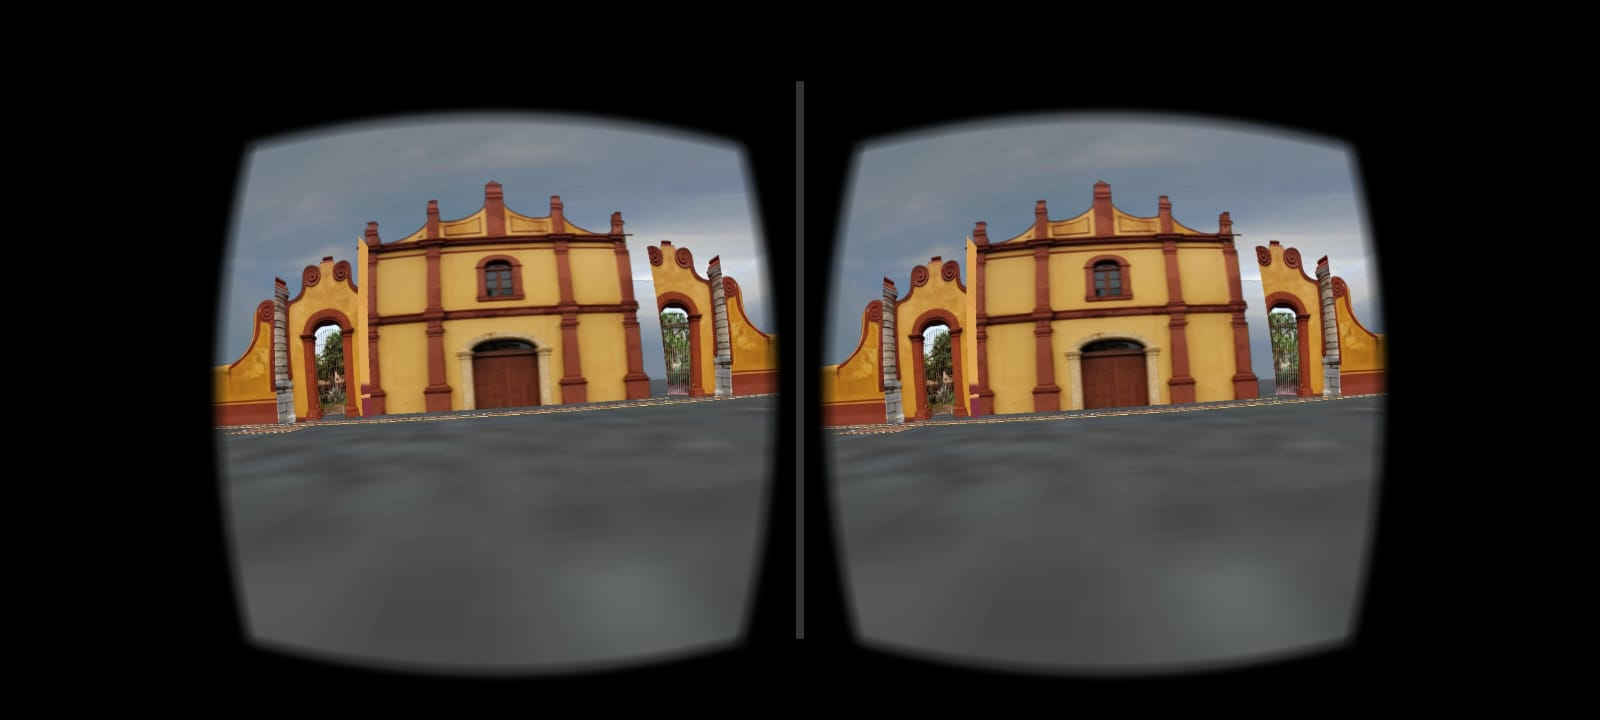
\includegraphics[width=0.95\columnwidth]{fig1.png}
\caption{Vista exterior del museo virtual dentro del visor estereoscópico.}
\label{fig:exterior}
\end{figure}

\section{Desarrollo Experimental}

La aplicación fue desarrollada en Android Studio y se organizó como un proyecto móvil con clases orientadas al renderizado de objetos, manejo de cámara, lectura de sensores y representación de la vista tipo Cardboard. Dentro del proyecto se identifican componentes relacionados con el dispositivo VR, distorsión óptica, seguimiento de cabeza, renderizado de objetos y carga de texturas.

\subsection{Estructura General del Proyecto}

El proyecto se compone de una actividad principal encargada de iniciar la vista VR y un conjunto de clases auxiliares para el renderizado. La escena del museo se presenta dos veces en pantalla, una para el ojo izquierdo y otra para el ojo derecho. Esta división permite simular una visualización binocular y resulta necesaria para el uso con visores móviles.

Entre los componentes principales se encuentran las clases de cámara, transformación, materiales, luz, objetos renderizables y lectura de recursos. También se incluyen clases relacionadas con el seguimiento de orientación, las cuales permiten que la escena responda al movimiento físico del dispositivo.

\subsection{Visor Estereoscópico}

El visor implementado presenta dos áreas de visualización separadas por una línea central. Cada área muestra la misma escena desde una perspectiva equivalente para simular el uso de un visor VR. Sobre la escena se coloca una máscara negra que deja visible únicamente la zona central de cada ojo, reduciendo la distracción de los bordes de la pantalla.

Este cambio permite que el usuario perciba la escena como si estuviera mirando a través de un visor. Además, el fondo negro ayuda a concentrar la atención en el museo virtual y mejora la presentación del recorrido.

\begin{figure}[H]
\centering
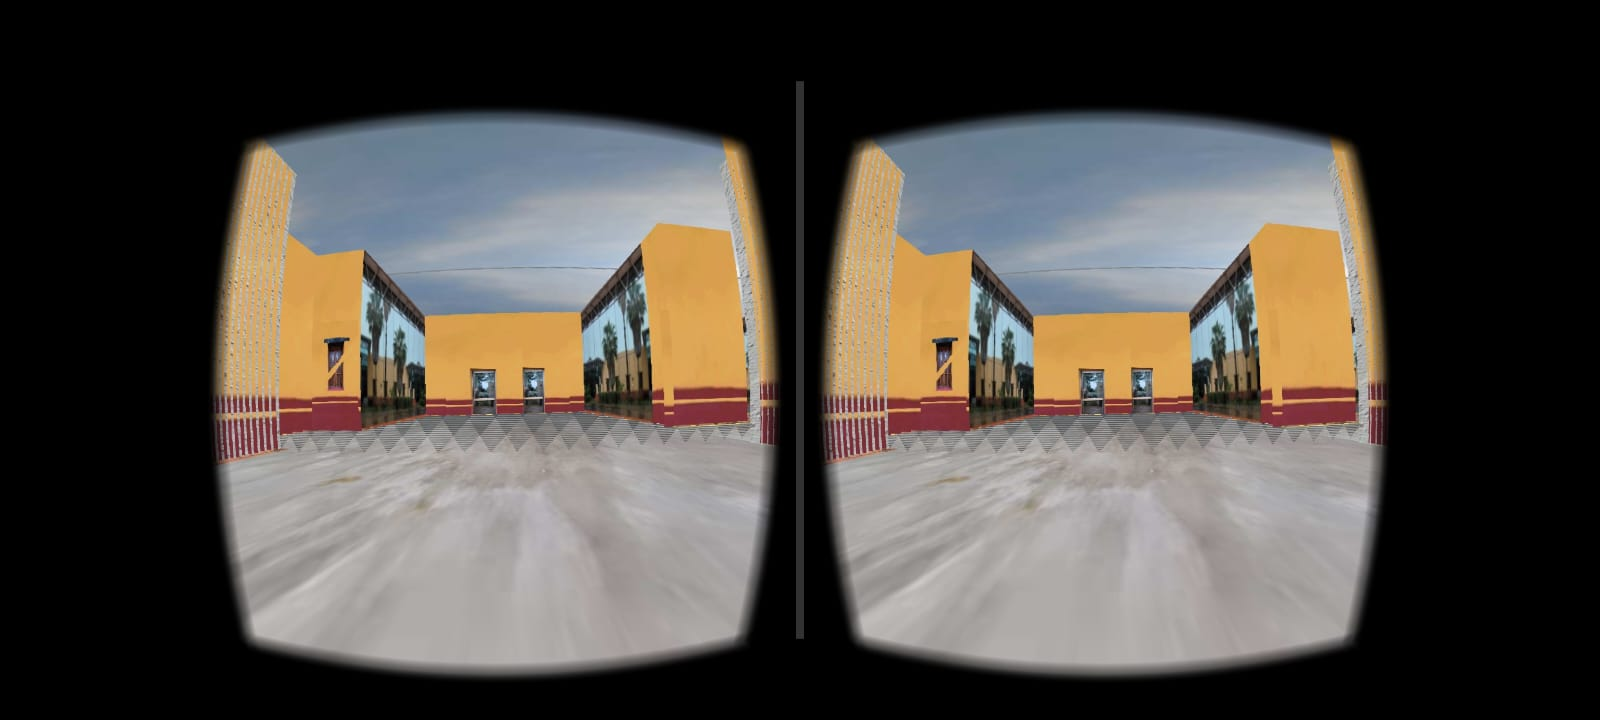
\includegraphics[width=0.95\columnwidth]{fig2.png}
\caption{Vista interna del museo virtual con el marco oscuro aplicado en ambas mitades de pantalla.}
\label{fig:interior}
\end{figure}

\subsection{Corrección de Navegabilidad}

Uno de los problemas principales del proyecto era que el usuario podía presentar movimientos no deseados al cambiar la orientación de la vista, especialmente al mirar hacia arriba. Para corregir este comportamiento, se ajustó la lógica de navegación para separar la rotación de la cabeza del desplazamiento del usuario dentro del plano del escenario.

La corrección consistió en evitar que el componente vertical de la mirada afectara directamente el avance dentro de la escena. De esta manera, el usuario puede observar hacia arriba o hacia abajo sin que la cámara se desplace fuera del plano del museo. El movimiento se mantiene principalmente sobre el plano horizontal, lo que hace que el recorrido sea más natural y estable.

\subsection{Renderizado de la Escena}

La escena del museo se renderiza con elementos arquitectónicos, texturas de suelo, paredes y áreas exteriores. El uso de texturas permite que el entorno tenga mayor realismo visual. Las pruebas muestran diferentes zonas del recorrido, incluyendo una fachada, un patio interior y una zona cercana al suelo con vegetación.

\begin{figure}[H]
\centering
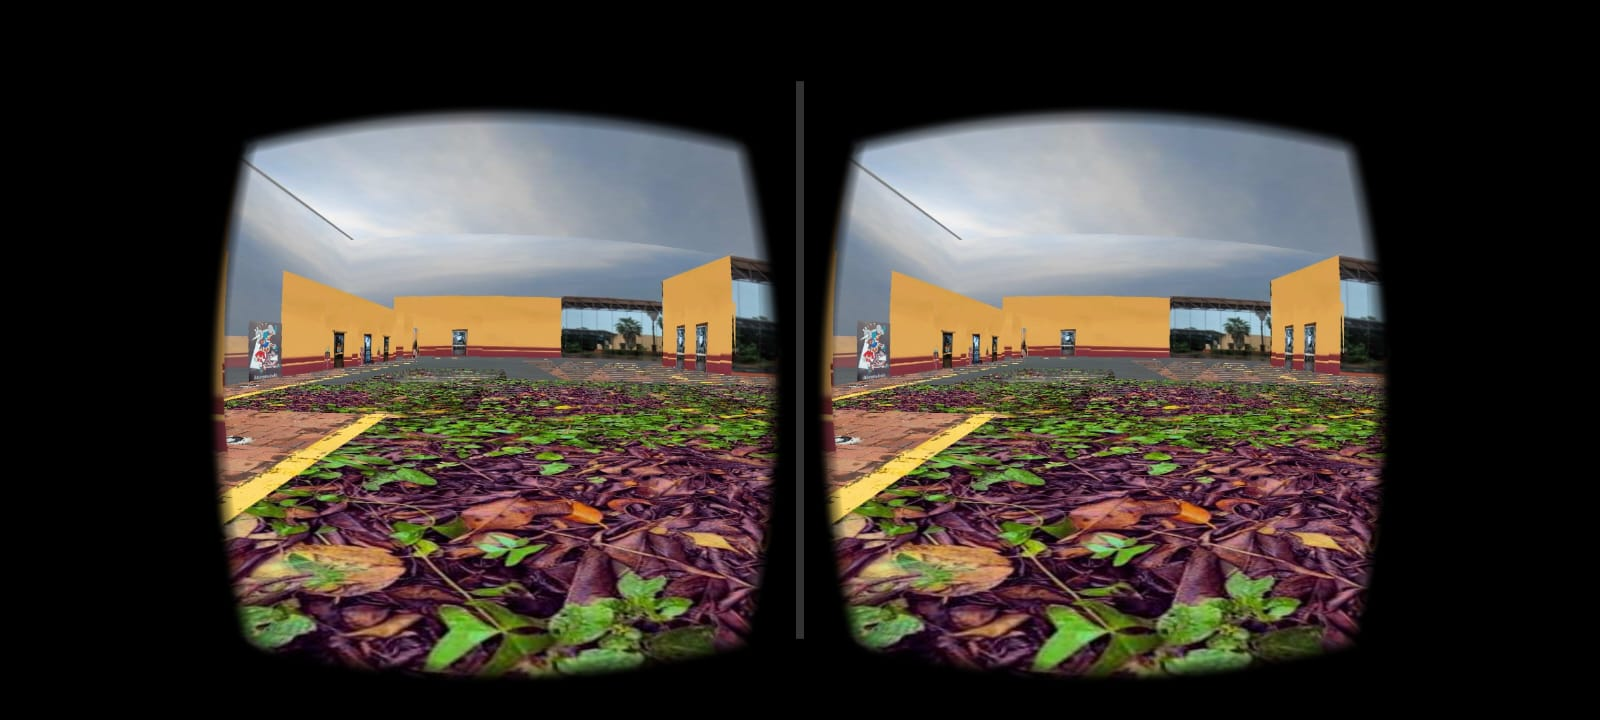
\includegraphics[width=0.95\columnwidth]{fig3.png}
\caption{Prueba de navegación dentro del entorno con vista baja hacia el suelo y elementos del escenario.}
\label{fig:suelo}
\end{figure}

\section{Resultados}

Las pruebas realizadas permitieron comprobar que el visor estereoscópico se muestra correctamente en pantalla, con dos vistas sincronizadas y una máscara negra que delimita el área de observación. La línea central divide las vistas y mantiene la separación visual necesaria para el formato VR.

La Figura \ref{fig:exterior} muestra la fachada del museo virtual con el visor aplicado. La escena se conserva visible dentro de cada área de observación y los bordes exteriores permanecen oscurecidos. La Figura \ref{fig:interior} presenta una zona interna del museo, donde se observa que el efecto del visor se mantiene durante el desplazamiento. Finalmente, la Figura \ref{fig:suelo} evidencia una prueba con orientación baja, útil para verificar que la cámara puede cambiar de dirección sin romper la visualización del plano.

\begin{table}[H]
\centering
\caption{Resultados de pruebas realizadas}
\label{tab:pruebas}
\begin{tabular}{p{0.28\columnwidth}|p{0.31\columnwidth}|p{0.25\columnwidth}}
\toprule
Prueba & Esperado & Obtenido\\
\midrule
Vista VR doble & Dos vistas separadas para cada ojo & Correcto\\
Marco del visor & Bordes negros y zona central visible & Correcto\\
Navegación horizontal & Movimiento estable en el plano del museo & Correcto\\
Movimiento vertical & Evitar salida del plano al mirar arriba & Correcto\\
Escena texturizada & Visualización del museo con texturas & Correcto\\
Separación central & Línea divisoria entre ambas vistas & Correcto\\
\bottomrule
\end{tabular}
\end{table}

\section{Conclusión}

Se desarrolló y ajustó satisfactoriamente una aplicación de museo virtual en Android con visualización estereoscópica tipo VR. El proyecto permitió integrar un visor oscuro con áreas visibles para cada ojo, conservar la división binocular de la pantalla y mejorar la presentación de la escena durante el recorrido.

También se corrigió el comportamiento de navegación para evitar que la orientación vertical provocara desplazamientos fuera del plano del escenario. Con ello, el usuario puede mirar hacia arriba o hacia abajo sin perder estabilidad en el recorrido. Las pruebas realizadas muestran que la aplicación presenta correctamente las vistas del museo, mantiene la máscara del visor y permite una navegación más controlada dentro del entorno virtual.

\begin{thebibliography}{00}

\bibitem{androiddevelopers} Google, ``Android Developers Documentation.'' [En línea]. Disponible: \url{https://developer.android.com}. Consultado el \specialdate\today.

\bibitem{androidopengl} Google, ``OpenGL ES on Android.'' [En línea]. Disponible: \url{https://developer.android.com/develop/ui/views/graphics/opengl}. Consultado el \specialdate\today.

\bibitem{androidsensors} Google, ``Sensors Overview.'' [En línea]. Disponible: \url{https://developer.android.com/develop/sensors-and-location/sensors/sensors_overview}. Consultado el \specialdate\today.

\bibitem{androidstudio} Google, ``Android Studio.'' [En línea]. Disponible: \url{https://developer.android.com/studio}. Consultado el \specialdate\today.

\bibitem{cardboard} Google, ``Google Cardboard.'' [En línea]. Disponible: \url{https://arvr.google.com/cardboard/}. Consultado el \specialdate\today.

\bibitem{opengles} A. Munshi, D. Ginsburg y D. Shreiner, \textit{OpenGL ES 3.0 Programming Guide}. Addison-Wesley Professional, 2014.

\bibitem{androidbignerd} B. Phillips, C. Stewart y K. Marsicano, \textit{Android Programming: The Big Nerd Ranch Guide}. Big Nerd Ranch Guides, 2022.

\bibitem{realtime} T. Akenine-Moller, E. Haines y N. Hoffman, \textit{Real-Time Rendering}. CRC Press, 2018.

\end{thebibliography}

\end{document}
